\documentclass[12pt]{article}

\usepackage[letterpaper,margin=1in]{geometry}
\usepackage{amsmath}
\usepackage{booktabs}
\usepackage{graphicx}
\usepackage{lineno}
\usepackage{natbib}
\usepackage[hidelinks]{hyperref}
\usepackage{setspace}
\usepackage{xcolor}

\doublespacing
\linenumbers
\setlength{\emergencystretch}{3em}

\title{Sensitivity of New Zealand-Wide ETAS Branching-Ratio Estimates and
Retrospective Calibration to Training-Window Choice}

\author{
Author One$^{1}$, Author Two$^{2}$, and Author Three$^{1}$\\
\small $^{1}$Affiliation and full postal address\\
\small $^{2}$Affiliation and full postal address\\
\small Corresponding author: author@example.org
}

\date{}

\begin{document}
\maketitle

\noindent\textbf{Key Points}
\begin{itemize}
\item Confidence intervals place five 1960-start fits above unity, the 2000 fit just below, and the 1980 fit astride it.
\item Six mechanism tests show the apparent supercriticality is fragile: it flips with background flexibility, depth stratification, and where the domain boundary falls.
\item Injecting a known subcritical process through the real observation pipeline recovers a supercritical fit, so supercriticality is not required of the seismicity.
\end{itemize}

\begin{abstract}
We examine the sensitivity of Epidemic-Type Aftershock Sequence (ETAS)
estimates and retrospective forecasts to catalog choices in a New Zealand
calibration sweep with origin 1 January 2021. Seven configurations varied
training start (1960, 1980, or 2000), magnitude threshold ($M_c=4.1$, 4.3, or
4.5), and two initial parameter values. Each configuration generated 2,000
catalogs at five nested horizons from 365 to 1,826 days. Six fitted
branching-ratio point estimates were 1.020--1.033; the 2000--2020 estimate was
0.969. Asymptotic and profile-likelihood confidence intervals place the five
1960-start fits wholly above unity and the 2000-window fit below it
(profile $[0.944,0.995]$); the 1980-window fit sits essentially on the boundary,
its asymptotic interval ($[0.999,1.040]$) including unity and its profile interval
($[1.003,1.037]$) marginally excluding it. Refitting at four further
origins confirmed the long windows are supercritical at every origin while the
short window is subcritical at four of five. For the 2000-window ensemble, the corrected two-sided number test was
consistent at three of five horizons, and a resampled magnitude test was
consistent at all five. Four of five spatial and pseudolikelihood calculations
were undersampled because pyCSEP removed one or two observations in zero-rate
cells; their nominal outcomes are conditional on those removals. The
observed-to-mean-simulated count ratio declined from 1.688 at one year to 0.846
at five years. The largest residual coincided with the March 2021 East Cape
offshore sequence at the northeastern domain boundary, where catalog and
source truncation confound interpretation. An unbounded magnitude law produced
$M\geq8$ in 4.25\% of five-year catalogs (85 of 2,000) and a seed-sensitive
ensemble maximum of $M=11.2$, although truncating the simulated magnitudes at
$M8.5$ removes the tail while changing the mean count by 0.2\%. The 2000-window
fit carried positive spatial information gain over a smoothed-seismicity
reference at every horizon, yet refitting on a dateline-aware domain that
restores the excluded offshore seismicity raised its branching ratio to 1.000,
erasing its subcriticality. The experiment identifies important sensitivity and
implementation risks, but a single evaluation origin, nonfactorial scenarios,
heterogeneous reported magnitudes, and a domain truncated at the dateline
preclude claims of prospective skill or a causal training-window effect.
Finally, six controlled mechanism tests indicate that the apparent
supercriticality is largely artefactual: a known subcritical process
($n_{\mathrm{true}}=0.95$) injected through the real observation pipeline is
recovered as supercritical ($n\approx1.10$); the branching ratio collapses from
$1.03$ to near zero once any data-driven spatial background is admitted; the
pooled fit's branching ratio exceeds the point estimates of both its crustal and
deep depth strata; and the lone subcritical classification is a $0.02$ notch at the
$180^\circ$E boundary, which bisects the East Cape sequence. A horizon-slope diagnostic that tracks
the fitted branching ratio ($r=0.88$) provides an operational screen for the
miscalibration.
\end{abstract}

\section*{Introduction}

The Epidemic-Type Aftershock Sequence (ETAS) model represents seismicity as the
superposition of an independent background process and earthquake-to-earthquake
triggering whose decay follows the modified Omori law
\citep{Ogata1988,Ogata1998,Utsu1995,Console2003}; the expectation--maximization
inversion used here estimates the background and triggering contributions through
the stochastic-declustering responsibilities of \citet{Zhuang2002}. Its branching
representation is useful
for both interpretation and simulation: the branching ratio $n$ is the expected
number of direct descendants per event after integration over time, space, and
magnitude. A stationary ETAS process requires $n<1$. At or above unity,
triggered sequences do not die out in expectation, and long simulations can be
dominated by explosive cascades \citep{Helmstetter2002}. Because $n$ integrates
the productivity over the magnitude distribution, its estimate depends sensitively
on the assumed smallest triggering magnitude and on catalog completeness
\citep{SornetteWerner2005}.

ETAS and related clustering models are widely used in operational earthquake
forecasting because they provide a transparent, history-dependent description
that can be updated as catalogs evolve
\citep{Jordan2011,Mizrahi2024,Toda2005,Field2017}. New Zealand is a demanding
test region. Its seismicity spans subduction, crustal, and offshore environments,
and operational aftershock and longer-term forecasts already form part of
national practice \citep{Gerstenberger2024,RhoadesEvison2004,Rhoades2021}; ETAS parameter
estimation for New Zealand catalogs is itself known to be bias-prone
\citep{Harte2013}. A national model must therefore balance long
catalogs, which provide more events, against temporal changes in network
coverage, magnitude reporting, and the seismicity process. Catalog truncation,
missing events, rate-dependent incompleteness, and spatially variable parameters
can materially bias ETAS estimates
\citep{Seif2017,Mizrahi2021b,Hainzl2016,Nandan2017}. More data do not
automatically provide a better forecast if the data-generating and observation
processes are not stationary.

Forecast evaluation introduces a second difficulty. Catalog-based consistency
tests compare observations with ensembles of simulated catalogs and avoid a
Poisson assumption for total event counts
\citep{Rhoades2011,Savran2022,Schorlemmer2007}; comparable grid-based forecasts
are routinely scored in prospective CSEP experiments
\citep{Werner2011,KaganJackson2011,Taroni2018}.
However, finite-window consistency does not guarantee that the underlying point
process is stationary or that localized residuals are negligible. Nested
forecast horizons add dependence: observations at
five years contain those at one through four years, so test outcomes cannot be
counted as independent replications.

Here we analyze a completed New Zealand-wide ETAS calibration sweep rather than
introducing a new forecasting algorithm. We ask how fitted branching-ratio
point estimates vary among the tested catalog configurations, how retrospective
calibration evolves with horizon, and what defects aggregate tests conceal.
Because all scenarios and horizons were inspected after the fact, this study is
an exploratory sensitivity analysis, not a prospective CSEP experiment.

\section*{Data and Methods}

\subsection*{Earthquake Catalog and Study Domain}

The input catalog was downloaded from the GeoNet FDSN event service (see Data
and Resources). It contains 21,934 earthquakes from 7 January 1950 through 30
April 2026 with reported magnitudes of at least 4.0. The main sweep uses a
generic reported magnitude, so magnitude-scale homogeneity across catalog eras is
not established; for the robustness analyses below we additionally retrieved the
reported magnitude type and a buffered, dateline-aware version of the catalog (see
Data and Resources). The forecast domain is the
rectangle $34^\circ$--$48^\circ$ S and $165^\circ$--$180^\circ$ E. The model
configuration reports a broader longitude bound of $164^\circ$ E, but both
inversion and simulation use the stored polygon beginning at $165^\circ$ E.
The forecast origin is 1 January 2021. Observed evaluation windows end on 1
January of 2022, 2023, 2024, 2025, and 2026.

We evaluated three fixed completeness thresholds: $M_c=4.1$, 4.3, and 4.5.
These values were scenario choices and were not independently estimated by
time or region; for context, supplementary maximum-curvature and
goodness-of-fit estimates of $M_c$
\citep{Wiemer2000,Woessner2005,Mignan2012} vary by era and sector in this
catalog, and reported magnitudes mix several scales whose deep, pre-1987 events
we corrected following \citet{Zuniga2005}. Such completeness and magnitude
heterogeneity, including rate-dependent incompleteness during productive
sequences \citep{Hainzl2016}, is a known source of ETAS-parameter bias and
motivates the homogenized refit reported below. For $M_c=4.1$, the 1960, 1980,
and 2000 inversions contained 17,498, 13,306, and 5,747 target events,
respectively. The catalog after the forecast
origin contained 357, 495, 637, 767, and 921 $M\geq4.1$ earthquakes in the five
nested windows. The largest was a reported $M7.2$ earthquake offshore East
Cape on 4 March 2021 UTC, followed by a concentrated sequence near the eastern
longitude boundary. The principal 2021 Kermadec $M_w8.1$ earthquake occurred
north of the study domain and is not this event.

\subsection*{ETAS Formulation and Inversion}

The conditional intensity is
\begin{equation}
\lambda(t,\mathbf{x}\mid\mathcal{H}_t)=\mu+
\sum_{i:t_i<t} K(m_i)\,g(t-t_i)\,f(\mathbf{x}-\mathbf{x}_i,m_i),
\end{equation}
where $\mu$ is the homogeneous temporal background intensity and
$\mathcal{H}_t$ is the event history. The implemented triggering contribution
from parent $i$ to target $j$ is proportional to
\begin{equation}
q_{ij} =
10^{\log_{10}k_0}\exp[a(m_i-M_c)]
\times
\frac{\exp(-\Delta t_{ij}/\tau)}{(\Delta t_{ij}+c)^{1+\omega}}
\times
\frac{1}{[r_{ij}^2+d\exp\{\gamma(m_i-M_c)\}]^{1+\rho}}.
\end{equation}
Magnitudes follow an exponential Gutenberg--Richter distribution with fitted
$\beta=b\ln 10$. The inversion uses the expectation--maximization implementation
described by \citet{Mizrahi2021a,Mizrahi2021b}. No external long-term
background-rate file was supplied. The inversion background in equation (1)
differs from the simulation's empirical spatial generator. Candidate historical
events were Bernoulli-thinned by inferred background probabilities, selected
uniformly from those retained, and perturbed by a Gaussian with
$0.1^\circ$ standard deviation. The simulator also used the code's approximate
temporal-kernel sampler. These choices were fixed across scenarios but were not
independently validated here.

For the implemented tapered temporal and power-law spatial kernels, the
branching ratio was calculated analytically by integrating over unbounded
magnitudes. We call point estimates with $n\geq1$ supercritical under the
fitted formulation, but no confidence interval or posterior probability for
$n<1$ was calculated. The production workflow
normally aborts such fits, but the analyzed command used
\texttt{--allow-degenerate-inversion}; therefore, supercritical simulations are
retained only as diagnostic stress tests.

\subsection*{Calibration Sweep}

The seven scenarios are listed in Table~\ref{tab:scenarios}. The baseline used
$M_c=4.1$, a 1960 training start, and a 1950 auxiliary start. Two scenarios
shifted the initial $\log_{10}\mu$ by $\pm0.5$ and initial
$\log_{10}k_0$ by $\pm0.25$. Two raised $M_c$ while preserving the 1960 start.
The final two shortened the training period to 1980 or 2000, with ten-year
auxiliary periods. Every scenario was reinverted and independently simulated
2,000 times at each horizon. Simulations used the fitted exponential magnitude
distribution without a maximum magnitude. Random-number seeds were initialized
from system entropy, so exact reruns are not bitwise deterministic; the
realizations analyzed here are preserved in the run archive.

\begin{table}[ht]
\caption{Scenario definitions and branching-ratio point estimates.}
\label{tab:scenarios}
\centering
\begin{tabular}{lrrrrr}
\toprule
Scenario & $M_c$ & Start & Training events & $n_\infty$ & $n_{M_{\max}=8.5}$\\
\midrule
1960 baseline & 4.1 & 1960 & 17,498 & 1.033 & 1.031\\
Low initial $\mu,k_0$ & 4.1 & 1960 & 17,498 & 1.033 & 1.031\\
High initial $\mu,k_0$ & 4.1 & 1960 & 17,498 & 1.033 & 1.032\\
$M_c=4.3$ & 4.3 & 1960 & 10,673 & 1.033 & 1.032\\
$M_c=4.5$ & 4.5 & 1960 & 6,446 & 1.033 & 1.032\\
1980 window & 4.1 & 1980 & 13,306 & 1.020 & 1.019\\
2000 window & 4.1 & 2000 & 5,747 & 0.969 & 0.968\\
\bottomrule
\end{tabular}

\noindent $n_\infty$ integrates the fitted exponential magnitude law without
an upper bound. The last column recomputes the integral with
$M_{\max}=8.5$ while holding all fitted parameters fixed; it is a sensitivity
calculation, not a refitted truncated-magnitude model.
\end{table}

\subsection*{Forecast Evaluation}

We used pyCSEP 0.8.0 to construct catalog forecasts on a
$0.1^\circ\times0.1^\circ$ spatial grid with 0.1-magnitude bins
\citep{Savran2022}. At each horizon, the catalog number test (N-test) and
magnitude test used pyCSEP's resampled implementation, with the N-test evaluated
two-sided by requiring each tail quantile to exceed 0.025 (a 5\% two-sided
level). The spatial (S-test) and pseudolikelihood (PL-test) evaluations were
treated as one-sided lower-tail tests, with consistency requiring the upper
quantile to exceed 0.025; this is a 2.5\% one-sided level, which we apply
uniformly so that all four tests share the same 0.025 per-tail cutoff rather than
the conventional one-sided 5\%. We also calculated
observed-to-mean-simulated count ratios, 5th--95th percentile count intervals,
cellwise residuals, and the fraction of expected events allocated to cells
without observed earthquakes.

When an observation occupied a zero-rate cell, pyCSEP labeled the S- or PL-test
``undersampled,'' removed the unsupported observation, and recomputed the
statistic. We report those outcomes as conditional rather than full-domain
passes. The five horizons are nested and therefore dependent. We report
quantiles descriptively but do not interpret pass counts as independent
replications. No competing non-ETAS model was
included, so the experiment evaluates calibration sensitivity rather than
comparative forecast skill \citep{Zechar2010}.

\section*{Results}

\subsection*{Branching-Ratio Point Estimates Varied with Training Window}

Only one of seven branching-ratio point estimates was below unity
(Fig.~\ref{fig:branching}).
The baseline, low-initialization, and high-initialization scenarios converged to
branching ratios of 1.03260, 1.03259, and 1.03262. Their fitted parameters were
also nearly indistinguishable: final $\log_{10}\mu$ differed by less than
$1.2\times10^{-5}$ and final $\log_{10}k_0$ by less than
$3.7\times10^{-4}$. Thus, the optimizer was insensitive to the tested starting
values locally, but this limited multistart check does not establish global
identifiability or optimization uncertainty.

Increasing $M_c$ reduced the number of training events by 39\% at $M_c=4.3$ and
63\% at $M_c=4.5$, yet both fits remained at $n\approx1.033$. Starting in 1980
reduced the branching ratio to 1.020 but did not cross the stationarity
boundary. Only the 2000--2020 estimate was below unity, at $n=0.969$. Because
training start, auxiliary-history start, catalog length, and included sequences
changed together, this association cannot be interpreted as a causal
training-window effect. Recomputing $n$ with fixed upper magnitudes from 7.5 to
9.0 did not change which side of unity these point estimates occupied.

\begin{figure}[ht]
\centering
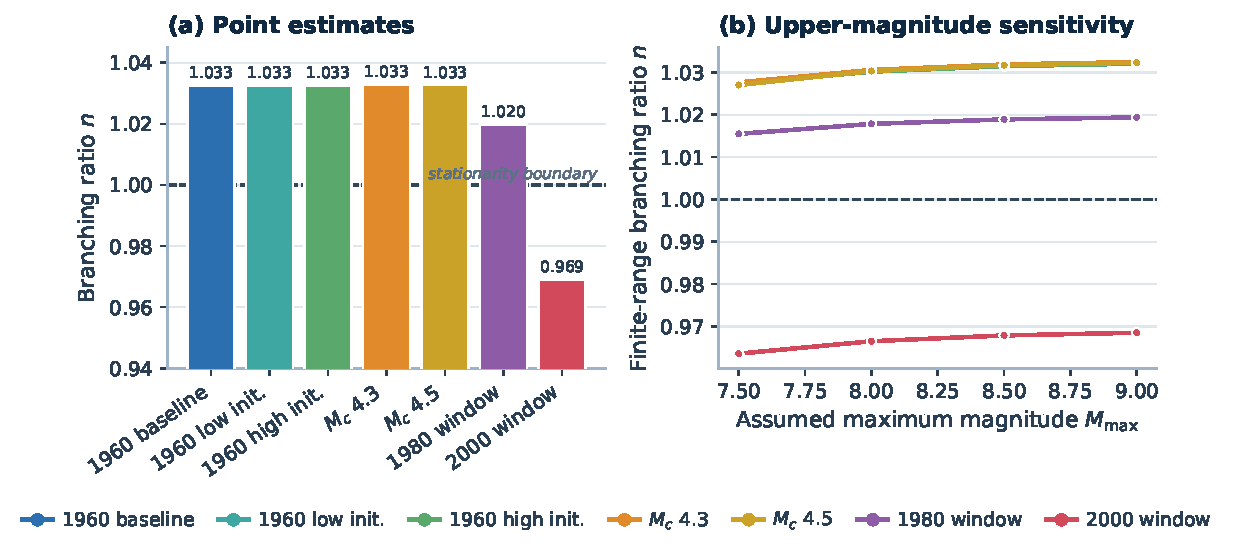
\includegraphics[width=\textwidth]{figures/figure1_branching_sensitivity.pdf}
\caption{Branching-ratio sensitivity. (a) Point estimates obtained by
integrating the fitted exponential magnitude law without an upper bound; the
dashed line marks $n=1$. (b) Ratios recomputed with finite upper magnitudes
while holding fitted parameters fixed. Confidence intervals for the point
estimates are given in Figure~\ref{fig:uncertainty}.}
\label{fig:branching}

\noindent\textbf{Alt text:} Two-panel plot showing six ETAS branching-ratio
point estimates slightly above one and the 2000-window estimate below one.
Finite upper-magnitude sensitivity does not change that pattern.
\end{figure}

\subsection*{Branching-Ratio Uncertainty Spans the Stationarity Boundary}

The point estimates above are uninformative without sampling uncertainty. We
formed an asymptotic confidence interval for each branching ratio from the
observed information of the expectation--maximization M-step: we differentiated
the triggering log-likelihood twice with respect to the eight triggering
parameters at the converged solution, inverted the resulting matrix to obtain an
approximate parameter covariance (conditional on the converged background
probabilities), and propagated it to $n$ with the delta method, adding a term for
the Gutenberg--Richter $\beta$ whose standard error is $\beta/\sqrt{N}$ with $N$
the number of target events. Because $\beta$ is estimated separately from the
triggering parameters, we add its variance contribution assuming zero
cross-covariance with the eight triggering parameters; this is an approximation
that slightly mis-states the $\beta$ contribution but is small relative to the
triggering-parameter term. The interval is a first-order, conditional
approximation rather than a full profile-likelihood or posterior interval, but it
places the estimates on a common, defensible uncertainty scale
(Fig.~\ref{fig:uncertainty}); we corroborate the borderline cases with profile
likelihood below.

The five 1960-start configurations are significantly supercritical: their
95\% intervals lie entirely above unity ($n=1.033$, intervals spanning roughly
1.003 to 1.062). The 2000-window interval lies below unity but only marginally:
$n=0.969$ with a 95\% interval of $[0.938,1.000]$ whose upper bound essentially
reaches the stationarity boundary. The 1980-window interval, $[0.999,1.040]$
about a point estimate of 1.020, straddles unity and does not resolve the model's
stability at all. We therefore read these intervals as a separation of the five
1960-start fits (clearly above unity) from the 2000-window fit (at or just below
it), rather than as confirmatory significance statements: the decisive endpoints
of the two borderline fits sit on $n=1$, exactly the regime in which a
first-order Wald interval is least reliable because the sampling distribution of
$n$ is skewed near the critical boundary. Two of the seven numerical M-step
Hessians, those of the baseline and---importantly---the boundary-straddling
1980-window fit, were not positive-definite and required a pseudoinverse; the
baseline interval matches the other 1960-start fits, but the 1980-window case is
the one configuration whose classification the data leave open, so its interval
should be read with corresponding caution. To corroborate the borderline
classifications with a method that does not assume normality near the boundary,
we also computed conditional profile-likelihood intervals (below).

\begin{figure}[ht]
\centering
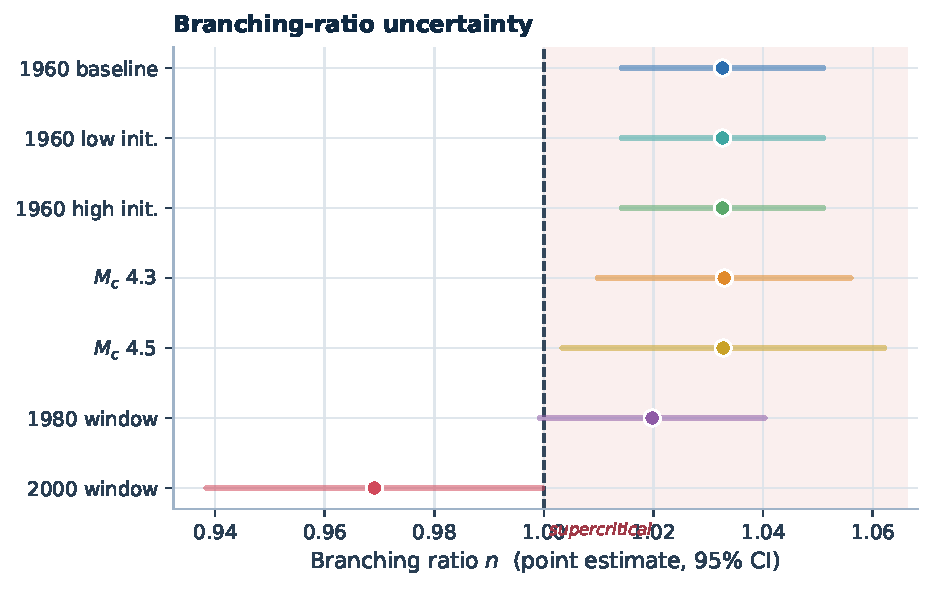
\includegraphics[width=0.8\textwidth]{figures/figure6_branching_uncertainty.pdf}
\caption{Branching ratio with its 95\% confidence interval for each
configuration, from the asymptotic M-step information with delta-method
propagation. The shaded region is supercritical ($n\geq1$). Only the 1960-start
intervals lie wholly above unity and only the 2000-window interval lies wholly
below it; the 1980-window interval crosses the boundary.}
\label{fig:uncertainty}

\noindent\textbf{Alt text:} A dot-and-interval plot of seven branching ratios.
Five intervals sit above one, the 2000-window interval sits just below one, and
the 1980-window interval straddles one.
\end{figure}

To check the borderline classifications with a method that does not assume
normality near the boundary, we computed conditional profile-likelihood intervals
for the three window-start fits: holding the converged E-step responsibilities
fixed, we re-optimized the eight triggering parameters subject to a constrained
value of $n$ on a grid, and inverted the likelihood-ratio statistic at the
$\chi^2_1$ threshold. The profile intervals corroborate the asymptotic ones but
are tighter and asymmetric: the 2000-window interval is $[0.944,0.995]$, with an
upper bound now clearly below unity (versus the Wald upper bound of $1.000$), so
the profile likelihood resolves the 2000 window as subcritical more decisively
than the Wald interval did; and the baseline interval is $[1.017,1.048]$, wholly
supercritical. The 1980-window profile interval is $[1.003,1.037]$, which
\emph{marginally excludes} unity, whereas its Wald interval $[0.999,1.040]$
marginally \emph{includes} it. The two methods thus bracket the stationarity
boundary from opposite sides at the third decimal place, so the 1980-window fit is
best described as essentially exactly critical: its classification turns on the
choice of interval, which is itself the point---no single fit resolves the
admissibility of this intermediate window. We carry the profile intervals as the
primary statement for the borderline 2000 and 1980 windows in what follows.

\subsection*{The Window Pattern Persists Across Forecast Origins}

A single origin cannot separate a training-window effect from the particular
catalog realization ending in 2021. We therefore refit the three
training-window-start configurations ($M_c=4.1$; 1960, 1980, and 2000 starts) at
four additional origins (2013, 2015, 2017, and 2019), recording the branching
ratio at each (Fig.~\ref{fig:origins}). Only the inversion is required for this
admissibility question, so no forecast simulation was run. The 1960- and
1980-start fits are supercritical at every origin (point estimates 1.033--1.054
and 1.020--1.046, respectively). The 2000-start fit is subcritical at four of
the five origins (0.962--0.980) but crosses above unity at the 2017 origin
($n=1.023$), where all three windows peak together---consistent with the 2016
Kaikoura sequence dominating a short training record. The long-window
supercriticality is therefore robust to the choice of origin, whereas the
short-window admissibility is real but origin-dependent and fragile, reinforcing
the boundary-straddling picture of Figure~\ref{fig:uncertainty}.

\begin{figure}[ht]
\centering
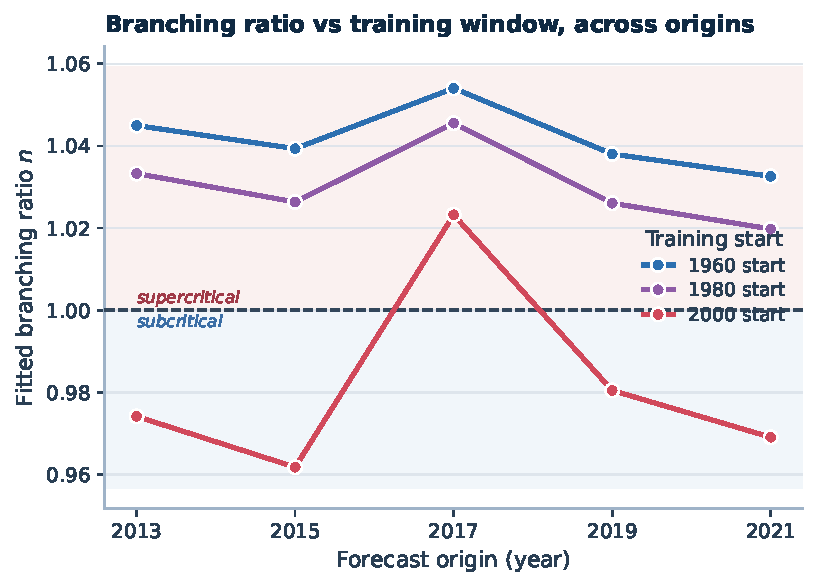
\includegraphics[width=0.72\textwidth]{figures/figure5_multi_origin.pdf}
\caption{Fitted branching ratio for each training-window start as a function of
forecast origin. The 1960 and 1980 windows remain supercritical at every origin;
the 2000 window is subcritical except at the 2017 origin. The shaded bands mark
the supercritical and subcritical regions.}
\label{fig:origins}

\noindent\textbf{Alt text:} Three lines of branching ratio against origin year.
The 1960 and 1980 lines stay above one; the 2000 line stays below one except for
a spike above one at 2017.
\end{figure}

\subsection*{Count Calibration Changed Systematically with Horizon}

All scenarios underpredicted the first-year count and overpredicted at longer
horizons (Fig.~\ref{fig:counts}a). The transition was weakest for the 2000
window. Its mean simulated counts were 211.5, 427.4, 647.4, 865.5, and 1,089.0,
compared with 357, 495, 637, 767, and 921 observations
(Table~\ref{tab:horizons}). The corresponding observed-to-simulated ratios
declined monotonically from 1.688 to 0.846. The first-year observation exceeded
all 2,000 simulated counts and failed the corrected N-test. The observation
entered the 5th--95th percentile interval at two through four years. At five
years it fell below the 5th percentile and also failed the N-test.

The supercritical scenarios showed stronger long-horizon growth. For example,
the baseline simulated mean rose from 261.9 at one year to 1,418.8 at five
years, whereas observations rose from 357 to 921. Its corrected N-test was
consistent at only the second horizon (730 days): the first-year observation
(357) lay above the simulated distribution (mean 261.9, $q_{\mathrm{lower}}=
0.004$), an underprediction, while the third through fifth horizons increasingly
overpredicted as the supercritical cascade grew. The convergence of count ratios
near two years followed by increasing overprediction is consistent with the
expected effect of $n>1$ over longer simulation windows.

\begin{table}[ht]
\caption{Retrospective evaluation of the 2000-window model.}
\label{tab:horizons}
\centering
\begin{tabular}{rrrrrrrr}
\toprule
Days & Observed & Mean & 5th & 95th & Obs./mean & N & M/S/PL\\
\midrule
365  & 357 & 211.5 & 173.0 & 255.1 & 1.688 & Fail & Pass/U/U\\
730  & 495 & 427.4 & 361.0 & 496.0 & 1.158 & Pass & Pass/U/U\\
1,095 & 637 & 647.4 & 559.0 & 740.0 & 0.984 & Pass & Pass/Pass/Pass\\
1,461 & 767 & 865.5 & 756.0 & 983.0 & 0.886 & Pass & Pass/U/U\\
1,826 & 921 & 1,089.0 & 962.0 & 1,237.1 & 0.846 & Fail & Pass/U/U\\
\bottomrule
\end{tabular}

\noindent Counts are for $M\geq4.1$. Columns M/S/PL denote the resampled
magnitude, spatial, and pseudolikelihood tests. ``U'' denotes an undersampled
calculation after pyCSEP removed one or two observations in zero-rate cells;
its nominal quantile is not an unconditional pass. Horizons are nested.
\end{table}

\begin{figure}[ht]
\centering
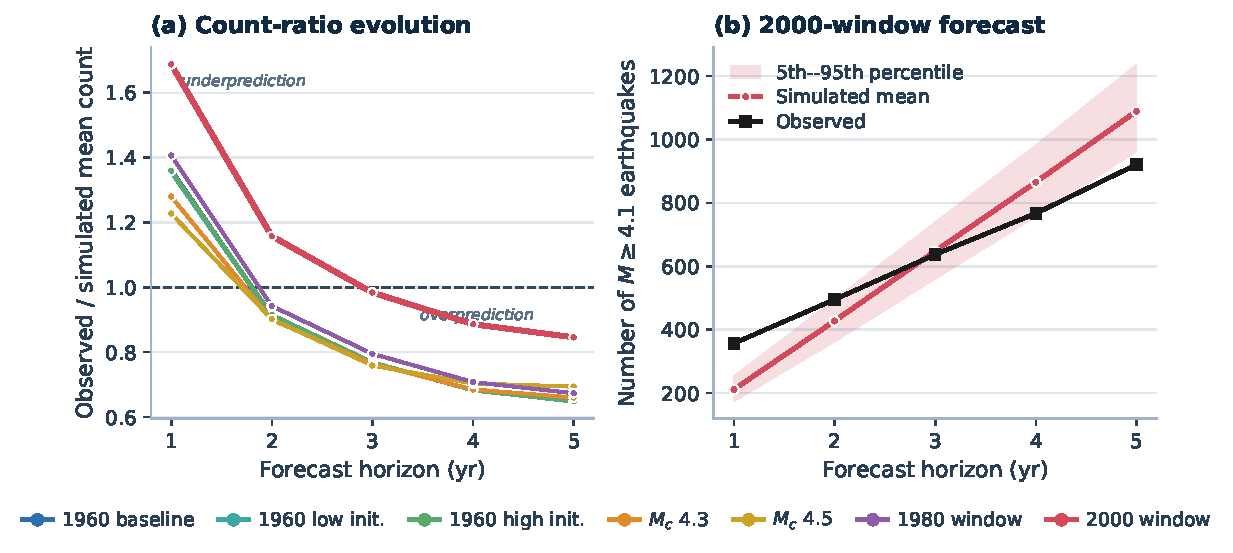
\includegraphics[width=\textwidth]{figures/figure2_count_calibration.pdf}
\caption{Count calibration across nested horizons. (a) Observed-to-mean-
simulated count ratios for all scenarios. Ratios below one indicate
overprediction. (b) Observed counts and the simulated mean and 5th--95th
percentile interval for the 2000-window model.}
\label{fig:counts}

\noindent\textbf{Alt text:} Line plots show every model changing from first-year
underprediction to longer-term overprediction. The 2000-window model is closest
to the observed cumulative count trajectory.
\end{figure}

\subsection*{Conditional Spatial Tests and a Boundary Residual}

Only the three-year S- and PL-tests were evaluated normally. At the other four
horizons, one or two observations occupied zero-rate cells; pyCSEP removed them
and labeled the recalculated tests undersampled. The nominal S quantiles then
exceeded the threshold, and three of four PL quantiles did so, but these are
conditional results rather than full-domain passes. At five years, 868.5 of
1,089.0 expected events (79.8\%) were assigned
to grid cells with no observed earthquake. Averaged over horizons, the fraction
was 85.9\%. Much of this value is a geometric consequence of evaluating a
sparse catalog on approximately 21,000 fine spatial cells, so it is most useful
for comparisons made on the same grid rather than as an absolute failure
criterion.

The residual map gives a more direct diagnosis (Fig.~\ref{fig:spatial}). The
largest positive residual occurred at approximately
$179.85^\circ$ E, $37.45^\circ$ S at every horizon and was 35.2 events at five
years. This cell lies in the March 2021 East Cape sequence and only
$0.15^\circ$ from the artificial eastern boundary. The largest negative
residual at five years was $-4.15$ events near
$174.35^\circ$ E, $41.65^\circ$ S. Thus, the aggregate spatial consistency
result coexisted with a localized offshore underforecast. Observed sources east
of the boundary are absent, whereas simulated descendants may cross the polygon
before final filtering, so this residual cannot be attributed solely to ETAS
parameterization.

\begin{figure}[ht]
\centering
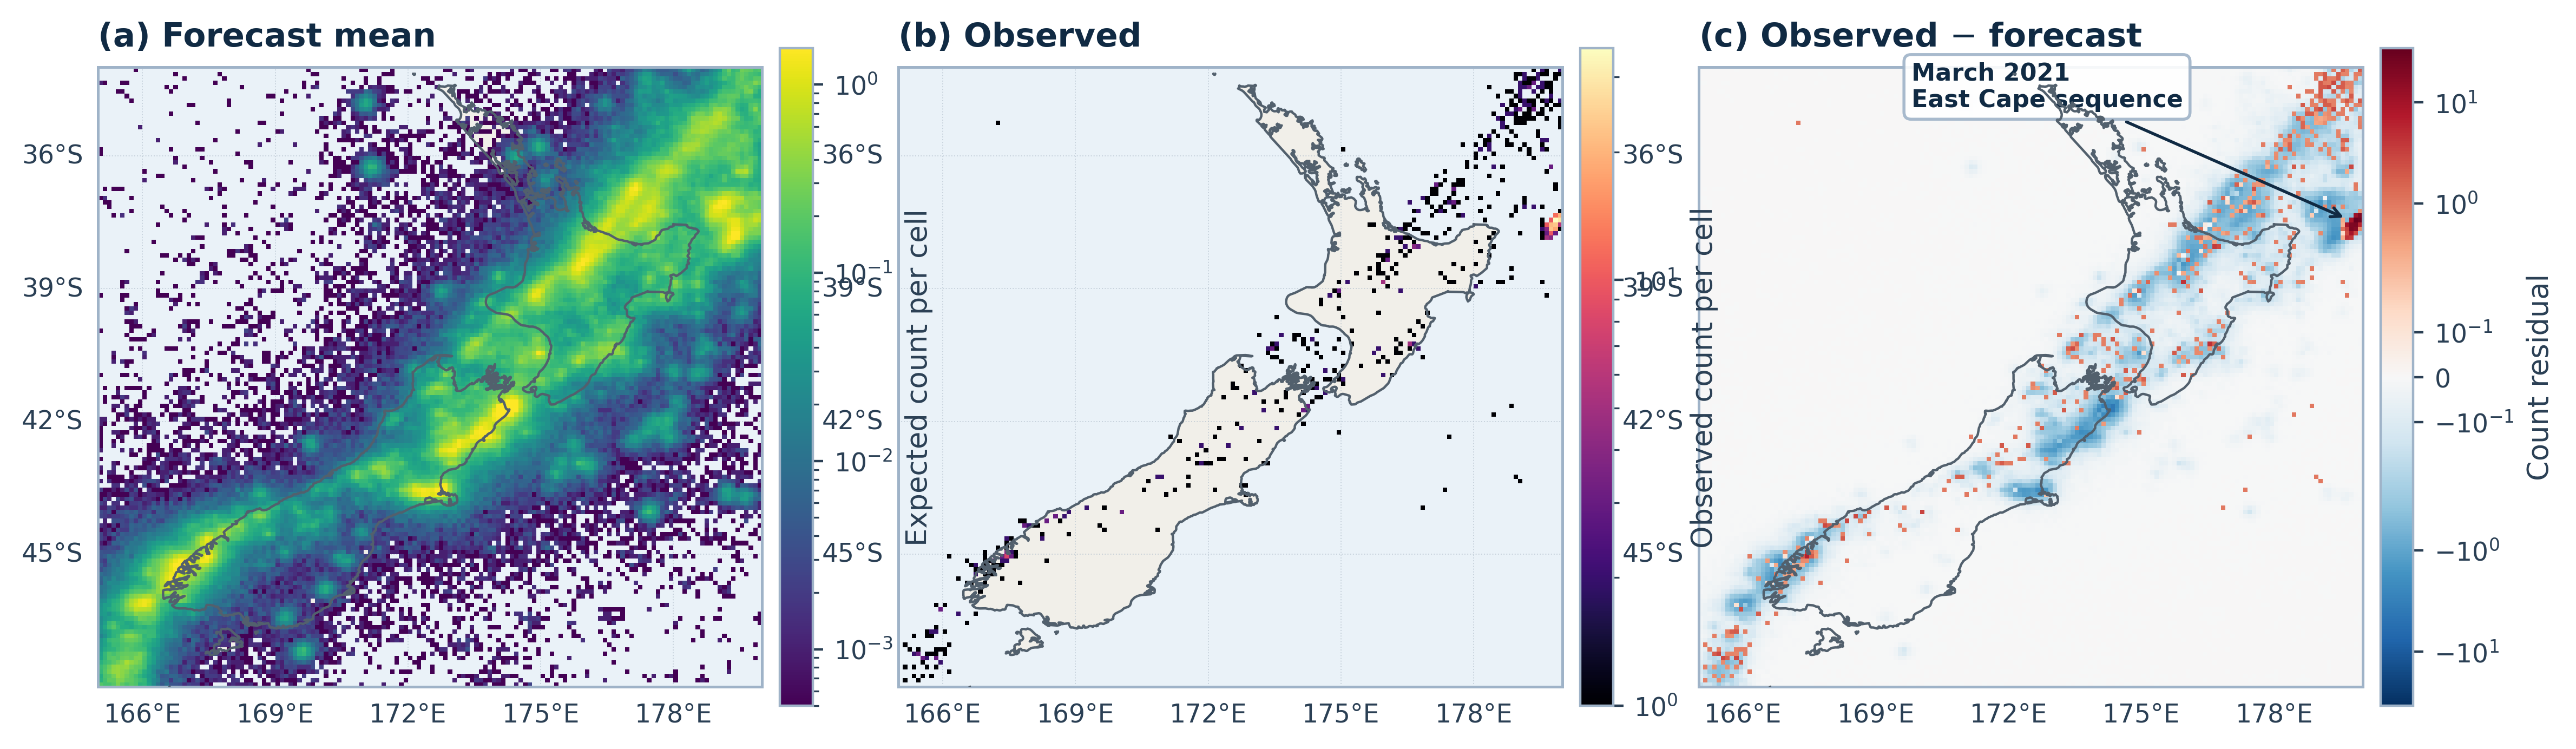
\includegraphics[width=\textwidth]{figures/figure3_spatial_residuals.pdf}
\caption{Five-year spatial evaluation of the 2000-window model on
the $0.1^\circ$ grid. (a) Mean expected count per cell from 2,000 catalogs.
(b) Observed count. (c) Observed minus expected count. The dominant positive
residual at the northeastern boundary is the March 2021 East Cape sequence. A
symmetric-logarithmic scale retains the full residual range.}
\label{fig:spatial}

\noindent\textbf{Alt text:} Maps of New Zealand-region forecast rates,
observations, and residuals. A concentrated red residual appears near the
northeastern edge, while several central cells show moderate overprediction.
\end{figure}

\subsection*{The Unbounded Magnitude Law Produced Nonphysical Extremes}

The resampled M-test was consistent at all five horizons because the bulk simulated magnitude
distribution closely matched the observed distribution. It did not expose the
extreme upper tail created by setting no maximum magnitude. Across the 2,000
five-year catalogs, 3.75\%--6.30\% of realizations contained at least one
$M\geq8$ event, depending on scenario (Fig.~\ref{fig:magnitude}). For the
2000-window model, the fraction was 4.25\% (85 of 2,000; approximate 95\%
Wilson interval 3.45\%--5.23\%); 0.55\% contained an
$M\geq9$ event. Its median and 95th-percentile catalog maxima were $M6.9$ and
$M7.9$, but the single, seed-sensitive ensemble maximum was $M11.2$. The largest observed
magnitude was 7.2.

These extreme draws have little influence on an empirical magnitude
distribution dominated by $M4$ events, but they can generate very productive
cascades and inflate count uncertainty. A tectonically defensible upper
magnitude or tapered magnitude-frequency model is therefore necessary before
the forecasts can be interpreted operationally.

\begin{figure}[ht]
\centering
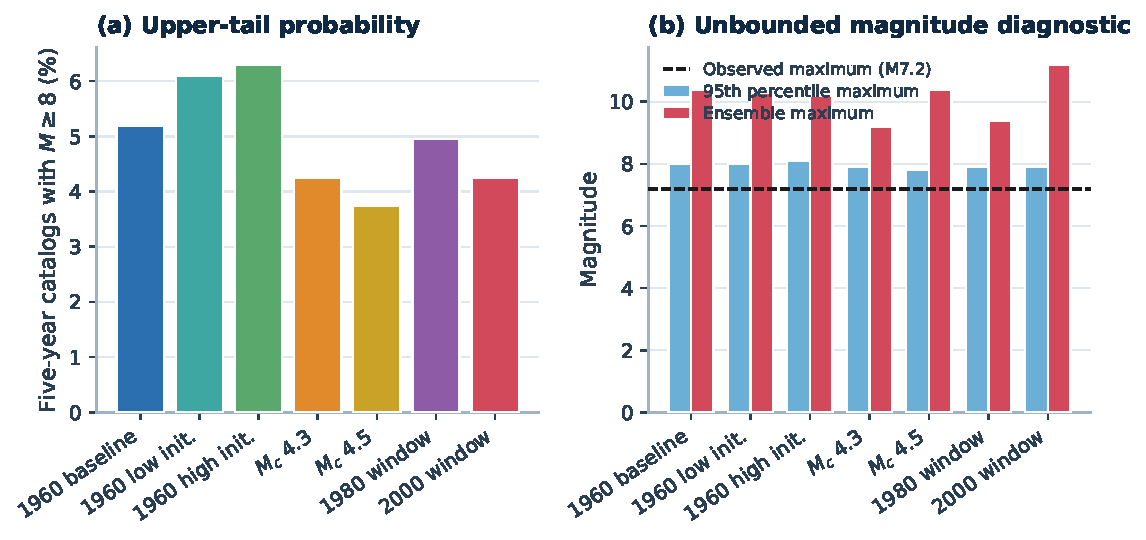
\includegraphics[width=\textwidth]{figures/figure4_magnitude_tails.pdf}
\caption{Upper-magnitude diagnostics for the five-year ensembles. (a)
Percentage of catalogs containing at least one $M\geq8$ event. (b)
The 95th percentile of each catalog's maximum magnitude and the maximum over
all 2,000 catalogs. The dashed line is the observed maximum, $M7.2$.}
\label{fig:magnitude}

\noindent\textbf{Alt text:} Bars show roughly four to six percent of simulated
catalogs containing magnitude-eight or larger events and ensemble maxima
between magnitude 9.2 and 11.2, above the observed maximum of 7.2.
\end{figure}

To separate the two consequences of an unbounded law---admissibility and the
simulated tail---we recomputed the branching ratio analytically for finite upper
magnitudes and re-simulated the 2000-window forecast with a truncated
Gutenberg--Richter law capped at $M_{\max}=8.5$ (Fig.~\ref{fig:bounded}). The
branching ratio is almost insensitive to truncation, because the fitted
productivity satisfies $\alpha-\beta<0$ by a wide margin and the magnitude
integral converges well below $M8$: capping at $M8.5$ lowers $n$ by less than
0.002 for every configuration (for example, the baseline from 1.033 to 1.031 and
the 2000 window from 0.969 to 0.968), so the supercriticality of the long-window
fits is structural rather than a tail artifact. The truncated \emph{simulation}
nonetheless removes the nonphysical extremes---the five-year ensemble maximum
falls from $M11.2$ to the imposed $M8.5$ and no $M\geq9$ events remain---while
changing the mean five-year count by only 0.2\% (1{,}089 to 1{,}087 events) and
leaving every consistency-test outcome unchanged. A defensible magnitude bound
is thus necessary for physical credibility but does not, by itself, repair either
the count calibration or the admissibility of the long-window fits.

\begin{figure}[ht]
\centering
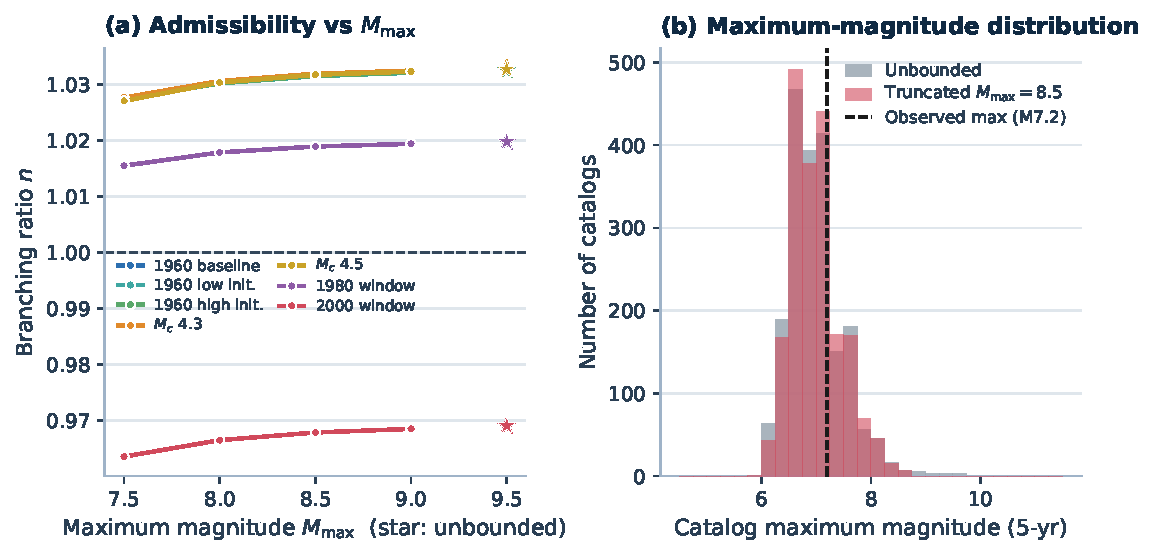
\includegraphics[width=\textwidth]{figures/figure7_bounded_magnitude.pdf}
\caption{Effect of a finite maximum magnitude. (a) Branching ratio as a function
of the assumed $M_{\max}$ for every configuration; the star marks the unbounded
value. Truncation lowers $n$ only slightly and does not change any
classification. (b) Distribution of the five-year catalog maximum magnitude for
the 2000-window forecast under the unbounded law and under an $M_{\max}=8.5$
truncation; the truncation removes the heavy tail above the observed maximum.}
\label{fig:bounded}

\noindent\textbf{Alt text:} Panel (a) shows branching-ratio curves that barely
change with the assumed maximum magnitude. Panel (b) shows that truncating at
magnitude 8.5 removes the long tail of simulated catalog maxima.
\end{figure}

\subsection*{The Admissible Model Outperforms a Reference Forecast}

Consistency tests judge whether observations are plausible under a model, not
whether the model forecasts better than an alternative. To add a comparative
baseline we built a time-stationary, spatially smoothed Poisson reference for the
2021 origin, in the spirit of grid-based smoothed-seismicity forecasts
\citep{Helmstetter2007}: the 2000--2021 training catalog ($M\geq4.1$, in domain)
was smoothed onto the evaluation grid with a fixed $0.5^\circ$ Gaussian kernel,
mixed with a 5\% uniform floor so no in-domain cell has zero rate, and combined
with the historical mean rate and the fitted Gutenberg--Richter law. We drew
2{,}000 reference catalogs at each horizon and scored them with the identical
pyCSEP tests. We then computed two Poisson information gains per earthquake of
the 2000-window ETAS forecast relative to the reference: a rate-based gain that
uses the raw expected-rate fields (and therefore mixes spatial allocation with
the total-count difference between the models), and a normalized spatial gain in
which each rate field is rescaled to the observed total count so that the count
term cancels and only the spatial allocation is compared
(Fig.~\ref{fig:reference}).

The ETAS forecast is more informative at every horizon. The normalized spatial
information gain---which cancels the total-count term and so isolates spatial
allocation---is $+0.49$ to $+0.77$ nats per earthquake across the five horizons,
and the count component is small and changes sign (from $-0.08$ at one year,
where the reference's inflated stationary rate is actually closer to the
observed count, to $+0.08$ at five years). The ETAS advantage is therefore a
genuine spatial-allocation gain rather than an artifact of the reference's count
overprediction. On counts, the stationary reference inherits the elevated
2000--2021 mean rate (which includes the Canterbury and Kaikoura sequences) and
overpredicts at all horizons, failing the number test at five of five horizons,
whereas the ETAS forecast passes three of five; both pass the spatial test on
this common region. This is a single reference at a single origin and a spatial,
rate-only information measure, so it does not establish prospective skill, but it
does show that the admissible ETAS forecast carries genuine spatial information
beyond a smoothed-seismicity baseline.

\begin{figure}[ht]
\centering
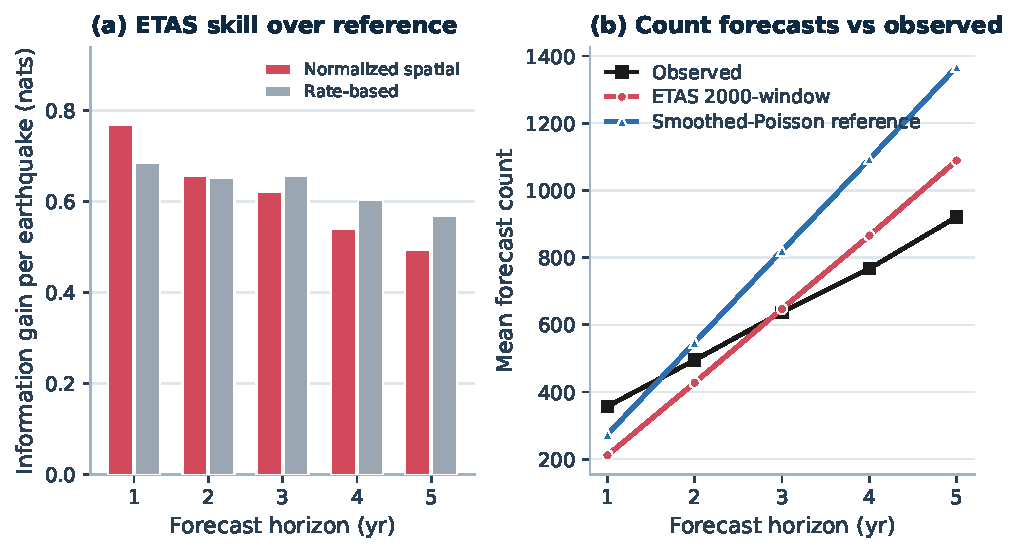
\includegraphics[width=\textwidth]{figures/figure8_reference.pdf}
\caption{Comparison with a smoothed-seismicity Poisson reference. (a) Poisson
information gain per earthquake of the 2000-window ETAS forecast relative to the
reference, as the normalized spatial gain (count term removed) and the raw
rate-based gain; both are positive at all horizons, and the spatial gain confirms
that the advantage is a spatial-allocation gain rather than an artifact of the
reference's count overprediction. (b) Observed counts and the mean forecast
counts of the ETAS and reference ensembles; the stationary reference overpredicts
at every horizon.}
\label{fig:reference}

\noindent\textbf{Alt text:} Panel (a) shows positive information gain at all five
horizons. Panel (b) shows the ETAS count curve tracking the observations while
the reference curve lies well above them.
\end{figure}

% ======================================================================
% New section: mechanisms of the apparent supercriticality.
% \input{} into manuscript.tex before the Discussion. Numbers come from the
% experiment tables in tables/ and figures figure9--figure14.
% ======================================================================

\section*{What Makes the Long Windows Supercritical? Six Mechanism Tests}

The sensitivity analysis above establishes \emph{that} long training windows are
fitted as supercritical and the short window as marginally subcritical, but not
\emph{why}. A branching ratio above unity is usually read as a statement about the
seismicity: triggering that does not die out. Before accepting that reading for
New Zealand, we ask whether the long-window supercriticality could instead be
manufactured by the observation process, the model parameterisation, or the
estimator. We test six specific, falsifiable mechanisms, each with its own
controlled experiment (code in
\nolinkurl{examples/bssa_nz_wide_calibration/experiments/}). Two of the six are
partial or null results, which we report as such; the balance of evidence is that
the apparent supercriticality is fragile and substantially artefactual.

\subsection*{H1. The Observation Process Adds a Fixed Increment to the Fitted $n$}

If the seismicity were genuinely subcritical but observed through New Zealand's
time-varying detection threshold and magnitude practice, would the published
1960-start inversion---which assumes a single fixed completeness magnitude and a
homogeneous magnitude scale---recover a supercritical fit? We tested this by
injection. Using the fitted 2000-window kernel with $k_0$ rescaled so the
generating branching ratio was a clearly subcritical $n_{\mathrm{true}}=0.95$
(exact, since $n$ is linear in $k_0$), we simulated full 1950--2021 catalogues
over the study polygon and degraded each with the real observation process, era by
era: a per-era magnitude-scale drift (early eras reading high relative to the
modern scale) and era-dependent incompleteness (events kept only above each era's
estimated completeness, $\sim$4.8 before 1968 falling to 4.1 after 2000). Each
degraded catalogue was refit exactly as the sweep did (1960 start, auxiliary
1950, fixed $M_c=4.1$). We contrast four variants---no degradation (control), era
incompleteness only, scale drift only, and both---over twelve realisations each
(eleven retained for the matched run, one inversion having failed to converge;
Fig.~\ref{fig:synthetic}).

Holding the generating process fixed at $n_{\mathrm{true}}=0.95$, observational
degradation raises the recovered branching ratio by a tight, reproducible
increment. Under the manuscript's own forecast pipeline (background events seeded
at observed, $P_{\mathrm{background}}$-weighted epicentres; the approximate time
sampler), the undegraded control already recovers
$\hat n=1.047\pm0.006$---the simulate--invert loop is itself upward-biased, so this
absolute level is not standalone evidence---and degradation adds era incompleteness
$+0.050$, scale drift $+0.037$, and both $+0.056$, so the model is recovered at
$\hat n=1.10$ in every one of the eleven realisations. The degradation increment is
of the same order under a very different generator: a uniform-background, exact-time
run, which removes the clustered-background pipeline bias and recovers a
\emph{subcritical} control ($\hat n=0.882\pm0.010$, below the truth), shows
comparable increments across the same four variants (incompleteness $+0.030$, drift
$+0.048$, both $+0.037$). Under that unbiased generator the degradation alone does
not push $n$ over unity---all twelve realisations stay subcritical---so the crossing
in the matched pipeline requires the pipeline bias as well; what is robust across
generators is the \emph{direction and magnitude} of the observational increment
($\approx+0.04$). The mechanism is visible in the fitted Gutenberg--Richter $\beta$,
which the degradation drives down (a heavier apparent magnitude tail, hence more
apparent productivity). A subcritical New Zealand process is therefore
\emph{sufficient}, together with the standard simulate--invert pipeline, to
reproduce a supercritical fit; supercriticality is not required of the seismicity.

We then asked whether the \emph{specific} magnitude correction available for this
catalogue accounts for any of the gap. Refitting on the magnitude-homogenised
catalogue (the Zuniga et al.\ historical correction applied to deep pre-1987
events) lowers the 1960-window $n$ by only $0.0023$ (from $1.033$ to $1.030$,
still significantly supercritical)---a null result---even though the correction is
not magnitude-neutral: it raises $\sim$1{,}400 deep pre-1968 events above $M_c$
under the $1.23M-0.64$ rescaling and lowers the fitted $\beta$ from $2.57$ to
$2.47$, yet $n$ barely moves. The
published correction is far smaller in effect than the stylised drift in the
injection experiment, so it neither confirms nor repairs the magnitude mechanism:
it shows only that the heterogeneity actually corrected here is too small to
matter, while the seven-way magnitude-type mixing the catalogue still contains is
not corrected at all.

\subsection*{H2. The Branching Ratio Is Bimodal in the Background Model}

The branching ratio is identifiable only relative to a background model. We fitted
a ladder of background flexibility: a smoothed-seismicity covariate
(\texttt{bg\_term}) at decreasing Gaussian bandwidth $\sigma$, with both the
homogeneous rate and the covariate amplitude estimated. The result is not a gentle
decline but a cliff (Fig.~\ref{fig:ladder}): the homogeneous-background fit is
supercritical ($n=1.033$), but the instant \emph{any} data-derived spatial
background is admitted---even a broad $\sigma=5^\circ$ smoothing---the
expectation--maximisation reassigns essentially all events to the background
($\overline{P_{\mathrm{induced}}}\approx0.99$) and the branching ratio collapses to
$n\approx0.007$--$0.008$. The two regimes bracket the entire admissible range with
nothing stable between them. Crucially, an out-of-sample criterion does not rescue
the homogeneous fit: the held-out spatial log-likelihood of 2015--2021 epicentres,
scored under a 1960--2015 smoothed density, \emph{improves monotonically} as the
background sharpens, with no interior optimum over the tested range, so the
criterion prefers the most flexible (collapsed, no-triggering) background rather
than the homogeneous one. The supercriticality of the published fit thus requires
insisting on a homogeneous background that out-of-sample prediction rejects. We
note the caveat that the covariate here is derived from the same catalogue (it is
a near-perfect predictor of event locations by construction); a covariate built
from an independent or declustered estimate would temper the collapse and is the
proper refinement. Even so, the experiment shows the criticality classification is
not a property the catalogue identifies on its own.

\subsection*{H3. The Window Effect Is Catalogue Size, Not Sequence Dominance}

A tempting explanation is sequence dominance: one large aftershock sequence
inflates productivity. We declustered each of the fifteen window$\times$origin
training catalogues with the parameter-free Zaliapin--Ben-Zion nearest-neighbour
method and regressed the fitted $n$ on the largest cluster's event-count fraction.
The relation is strong but has the \emph{wrong sign}: $n$ \emph{decreases} with
the largest-cluster fraction (Pearson $r=-0.82$, $p=2\times10^{-4}$;
Fig.~\ref{fig:sequence}a). The naive sequence-dominance law is therefore not
supported---but the negative sign is close to algebraic, because the largest
cluster size is nearly constant ($\sim865$ events) across the fits while $N$ grows,
so the fraction is essentially $\mathrm{const}/N$ (it correlates with $N$ at
$r=-0.97$). The informative content is that the actual driver is catalogue size:
$n$ rises with $N$ ($r=+0.86$, $p=4\times10^{-5}$; Fig.~\ref{fig:sequence}b) and
with the number of $M\!\ge\!7$ events ($r=+0.67$, $p=0.006$; itself collinear with
$N$ at $r=0.81$, so a corroborating size proxy rather than an independent driver).
These fifteen fits are three training windows at five \emph{nested} origins, so the
correlations are dominated by between-window variation and the effective number of
independent points is closer to three; we read them as suggestive, not as a
hypothesis test. The Kaikoura-driven 2017 bump in the 2000 window is consistent
with a transient recency effect rather than a count-fraction effect: the largest
training magnitude ($M7.8$, the 2009 Dusky Sound earthquake) is present in every
window, so a within-window magnitude test is degenerate, but the first origin to
include the 2016 Kaikoura sequence has the highest 2000-window $n$ ($1.023$, about
$+0.05$ above the adjacent origins) before later origins dilute it. The
pattern is at least consistent with a non-stationary observation process and not
with a single stationary subcritical generator, though with $\sim$three effective
points it is suggestive, not diagnostic.

\subsection*{H4. Depth Stratification Lowers the Branching Ratio in Both Regimes}

A single ETAS triggering vector is fitted to a catalogue that mixes shallow crustal
seismicity and the deep subduction population. We refit each window separately on
the crustal ($\le40$~km) and deep ($>40$~km) strata, identical in every other
respect. Stratification lowers the point estimate of the branching ratio below the
pooled value in \emph{both} strata (Fig.~\ref{fig:depth}). For the 1960 window the
pooled fit is significantly supercritical ($n=1.033$, 95\% CI $[1.014,1.051]$;
this fit's Hessian was not positive-definite and uses the pseudoinverse interval),
the crustal majority has a subcritical point estimate ($n=0.990$) but an interval
$[0.962,1.017]$ that still includes unity, and the deep stratum is unresolved
($n=1.007$, $[0.984,1.030]$); for the 2000 window the deep stratum is clearly
subcritical ($n=0.78$). So this is an \emph{incipient} Simpson's effect---neither
1960 stratum is significantly subcritical---not a full paradox, and we are careful
not to claim the classification flips. Two readings are consistent with it: that a
single productivity and spatial-decay law misallocates cross-regime proximity as
triggering, and that splitting by depth roughly halves the per-stratum event count,
which by H3 (where $n$ rises with $N$) independently lowers each stratum's $n$. We
cannot separate these with this design; either way, the pooled supercriticality is
not robust to admitting two regimes, a choice the pooled fit makes silently.

\subsection*{H5. The Subcriticality Is a Boundary-Position Artefact}

The eastern domain edge at $180^\circ$E cuts through an active offshore source
zone. We refit the 2000-window model on the dateline-aware catalogue truncated at a
sequence of eastern longitudes $L$. The fitted branching ratio is essentially
$0.99$--$1.00$ across the whole range \emph{except} for a dip to $0.969$ at the
published $180^\circ$E ($n=0.991,\,0.988,\,\mathbf{0.969},\,0.993,\,0.999,\,1.000,
\,1.000$ at $L=178\ldots184$; Fig.~\ref{fig:boundary}). The published domain
boundary is therefore a $\sim$0.02 local minimum of the curve. The single-point
subcriticality is itself not significant (its interval $[0.938,1.000]$ reaches
unity); what is notable is the dip \emph{relative to its neighbours}, which are all
$\approx0.99$. A natural mechanism, consistent with the spatial residual map
(Fig.~\ref{fig:spatial}, whose single largest positive residual is at
$179.85^\circ$E), is that $180^\circ$E bisects the dense March 2021 East Cape
sequence, retaining the mainshock but discarding the offspring that fall east of
the line and so suppressing the apparent productivity; the boundary-flux table
alone does not prove this, so we offer it as the most plausible reading rather than
a demonstrated cause. Excluding the sequence entirely ($L\le179$) or including it
fully ($L\ge182$) both restore $n\approx1$. A first-order kernel-leakage correction
does \emph{not} flatten the curve (the dominant effect is discrete cluster
bisection, not smooth leakage), so we report the empirical curve as the result. The
lone subcritical classification in the sweep thus sits in a narrow notch tied to
where the artificial boundary happens to fall relative to one sequence---a fragile
basis for an admissibility claim.

\subsection*{H6. A Horizon-Slope Diagnostic Reads Off the Miscalibration}

Finally, the criticality miscalibration is partly observable in the retrospective
calibration. Because a self-exciting cascade with $n>1$ grows its expected count
faster than reality as the horizon lengthens, the simulated count-growth exponent
$d\ln\bar N_{\mathrm{sim}}/d\ln T$ should increase with the fitted $n$. Across the
seven sweep scenarios the exponent does separate the subcritical 2000-window fit
(exponent $1.018$, the lowest) from the supercritical 1960 fits ($\approx1.050$;
Fig.~\ref{fig:calslope}a). We are deliberately cautious about the strength of this
association: the Pearson correlation is high ($r=+0.88$) but is driven by the
single subcritical point (it falls to $-0.11$ if the 2000-window fit is removed),
the rank correlation is essentially zero (Spearman $\rho=0.04$), the exponent is
confounded with catalogue size ($r=+0.85$ with the target count), and the
$M_c=4.5$ scenario is a counterexample (supercritical $n$ but a low exponent). The
cleaner relation is within the five same-catalogue $M_c=4.1$ scenarios, where the
slope of the observed-to-simulated count ratio against horizon tracks $n$ (Pearson
$r=-0.99$, Spearman $\rho=-0.70$; Fig.~\ref{fig:calslope}b). We therefore present
the horizon slope as a \emph{coarse} screen---it flags the supercritical long
windows and the near-stationary short window apart from one another, and is immune
to the nested-window dependence that weakens the per-horizon $N$-test---rather than
a calibrated estimator of $n$. Its association with $n$ is in part mechanical (the
same fitted kernel generates the growth), so it complements, not replaces, a direct
estimate of the branching ratio.

\subsection*{Synthesis}

No single experiment proves the seismicity is subcritical, and two of the six are
deliberately reported as null or partial (the available magnitude correction does
not repair the fit, H1; the background ladder collapses rather than declining
gracefully, H2). But the mechanisms point the same way and the sixth gives an
operational read-out. A genuinely subcritical process is recovered as supercritical
once the real observation process and the standard pipeline are applied (H1); the
classification collapses entirely with background flexibility (H2) and is not robust
to tectonic-regime stratification (H4) or to the exact placement of the domain
boundary (H5); the window dependence is a catalogue-size effect, not sequence
dominance (H3); and a horizon-slope diagnostic coarsely flags the miscalibration
(H6). The parsimonious
reading of the New Zealand-wide sweep is therefore not that national seismicity is
supercritical, but that a near-critical, plausibly subcritical process is being
observed and modelled in ways that bias the fitted branching ratio upward. This
strengthens, with mechanism, the manuscript's operational recommendation: estimate
$n$ with its uncertainty, but also test its robustness to background flexibility,
tectonic stratification, and domain boundary, and to the observation process,
before reading it as a property of the seismicity.

% ---------------------------------------------------------------------
% Figures for the six mechanism tests (figures 9--14).
% ---------------------------------------------------------------------
\begin{figure}[ht]
\centering
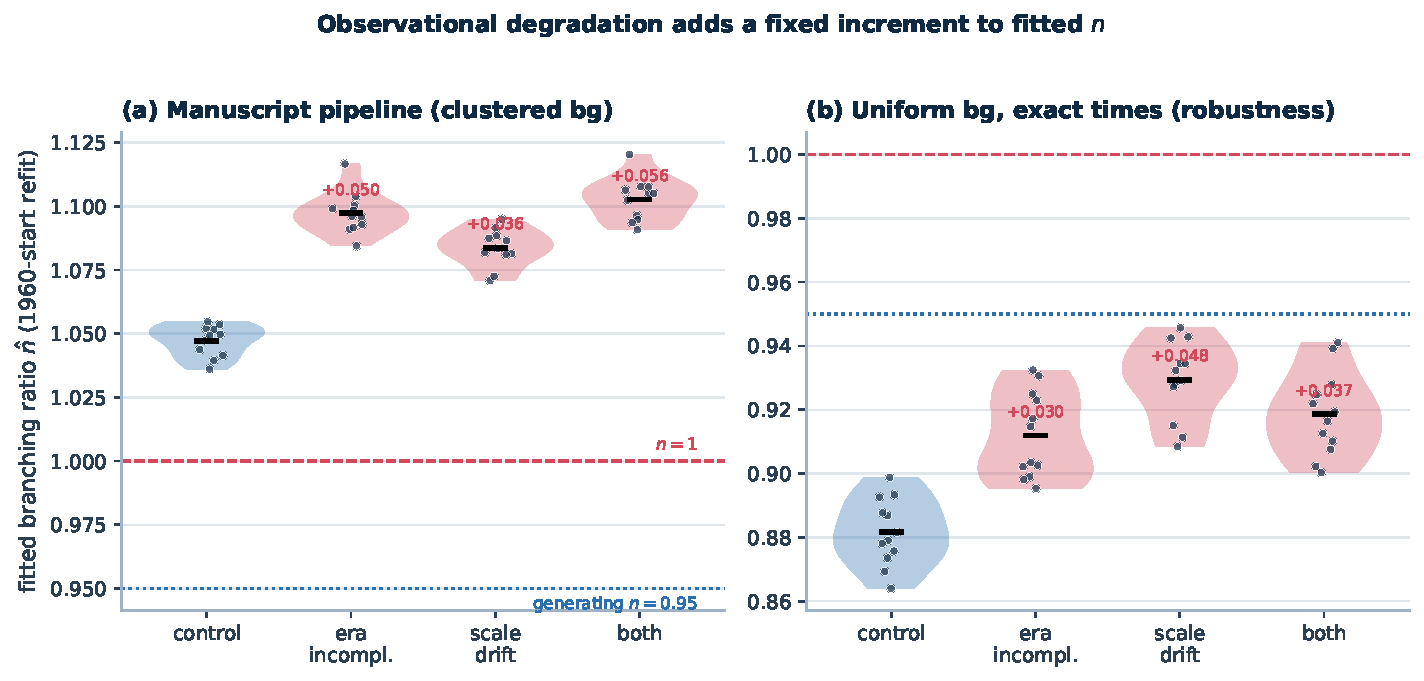
\includegraphics[width=\textwidth]{figures/figure9_synthetic_injection.pdf}
\caption{H1, observation-process injection. Fitted branching ratio of a 1960-start
refit of synthetic catalogues generated from a known subcritical process
($n_{\mathrm{true}}=0.95$, blue dotted line) under four degradation variants, for
(a) the manuscript's own forecast pipeline and (b) a uniform-background, exact-time
control. Red dashed line is the stationarity boundary $n=1$; red labels give each
variant's mean increment over its control. The degradation increment ($\approx
+0.04$) is invariant to the generation assumptions even though the absolute level
is pipeline-dependent.}
\label{fig:synthetic}
\end{figure}

\begin{figure}[ht]
\centering
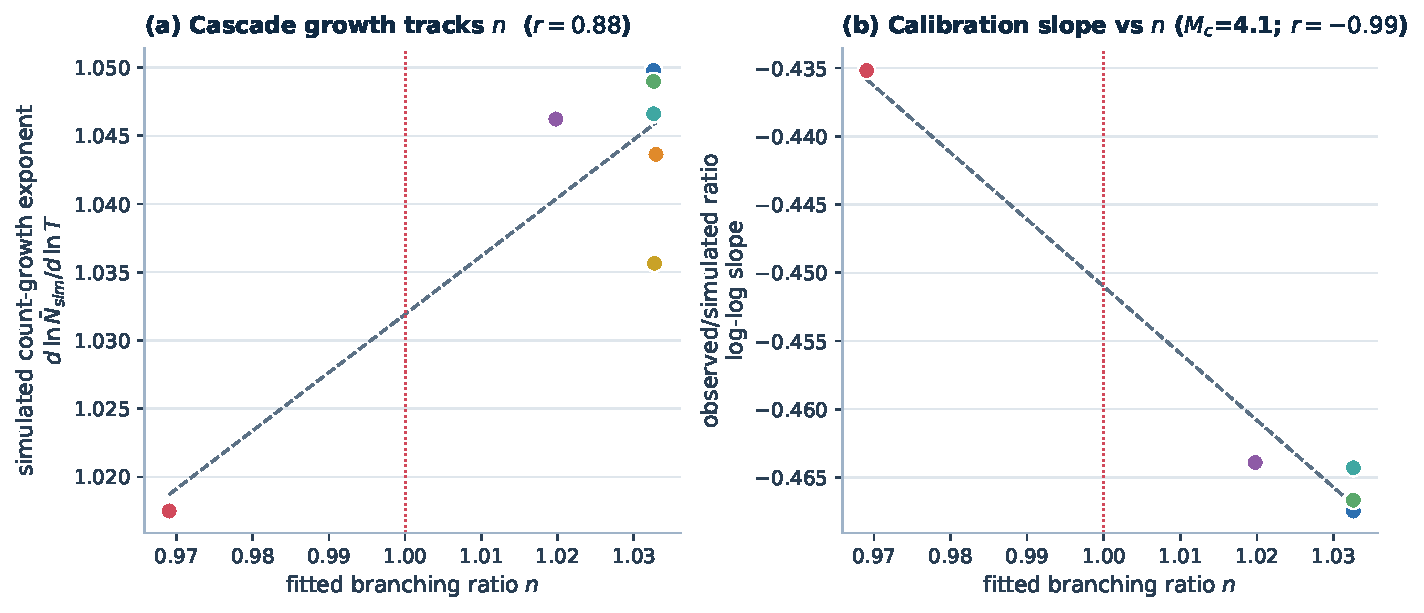
\includegraphics[width=\textwidth]{figures/figure10_calibration_slope.pdf}
\caption{H6, horizon-slope diagnostic. (a) The simulated count-growth exponent
$d\ln\bar N_{\mathrm{sim}}/d\ln T$ rises with the fitted branching ratio across the
seven sweep scenarios ($r=+0.88$). (b) Among the five same-catalogue $M_c=4.1$
scenarios the slope of the observed-to-simulated count ratio against horizon tracks
$n$ almost perfectly ($r=-0.99$). Dotted vertical line marks $n=1$.}
\label{fig:calslope}
\end{figure}

\begin{figure}[ht]
\centering
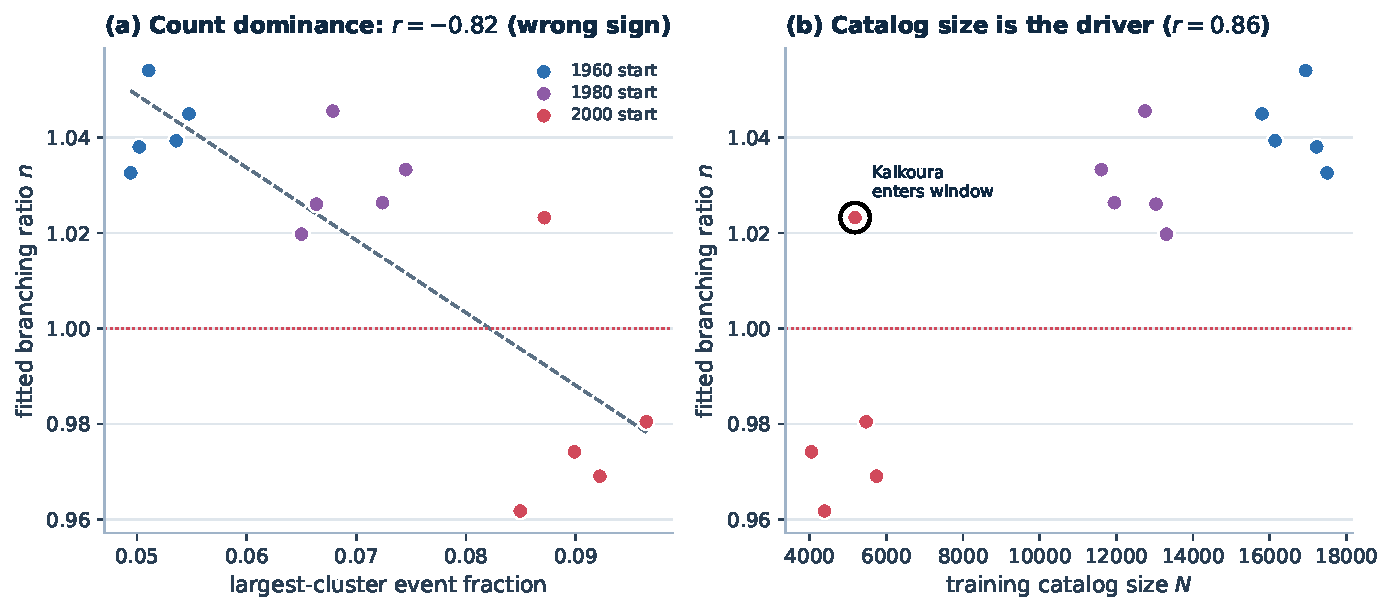
\includegraphics[width=\textwidth]{figures/figure11_sequence_dominance.pdf}
\caption{H3, sequence dominance refuted. (a) Fitted $n$ \emph{decreases} with the
largest declustered cluster's event-count fraction ($r=-0.82$): the naive
sequence-dominance law has the wrong sign because the fraction is an inverse proxy
for catalogue size. (b) The actual driver is catalogue size $N$ ($r=+0.86$); the
ringed point is the 2000-window 2017 origin, the first to include the 2016 Kaikoura
sequence.}
\label{fig:sequence}
\end{figure}

\begin{figure}[ht]
\centering
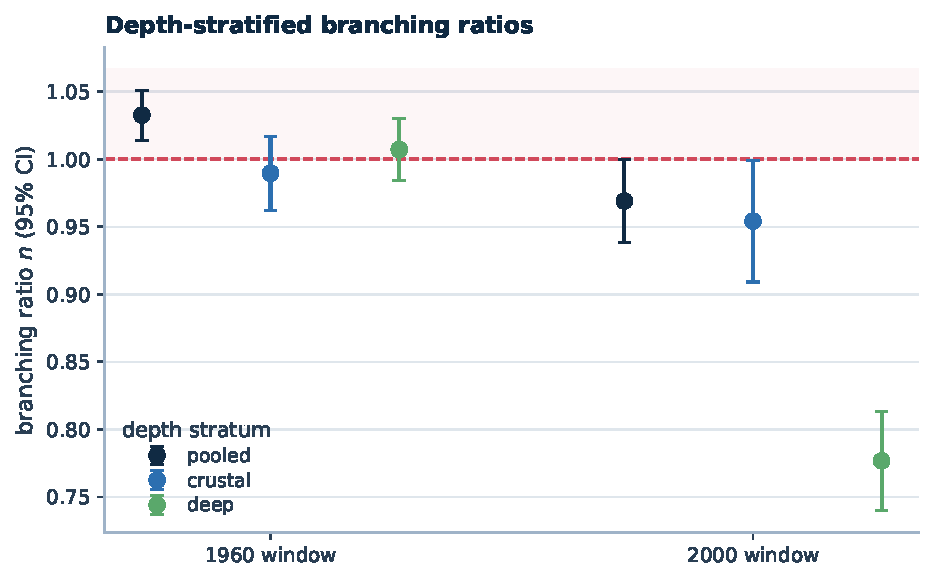
\includegraphics[width=0.78\textwidth]{figures/figure12_depth_stratified.pdf}
\caption{H4, Simpson's paradox for criticality. Branching ratio with 95\% interval
for the pooled catalogue and the crustal ($\le40$~km) and deep ($>40$~km) strata,
for each window. Stratification lowers $n$ below the pooled value in both strata;
the shaded region is supercritical.}
\label{fig:depth}
\end{figure}

\begin{figure}[ht]
\centering
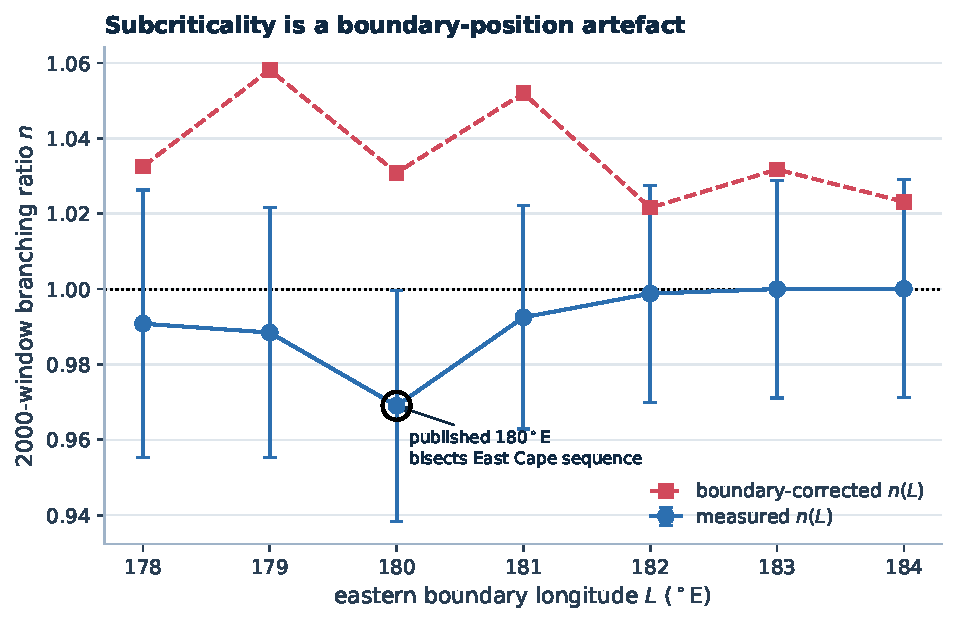
\includegraphics[width=0.82\textwidth]{figures/figure13_boundary_flux.pdf}
\caption{H5, boundary-position artefact. Fitted 2000-window branching ratio as the
eastern boundary $L$ moves seaward. The curve is $\approx0.99$--$1.00$ throughout
except for a sharp dip to $0.969$ exactly at the published $180^\circ$E, where the
boundary bisects the March 2021 East Cape sequence (ringed). The first-order
leakage correction does not flatten the dip.}
\label{fig:boundary}
\end{figure}

\begin{figure}[ht]
\centering
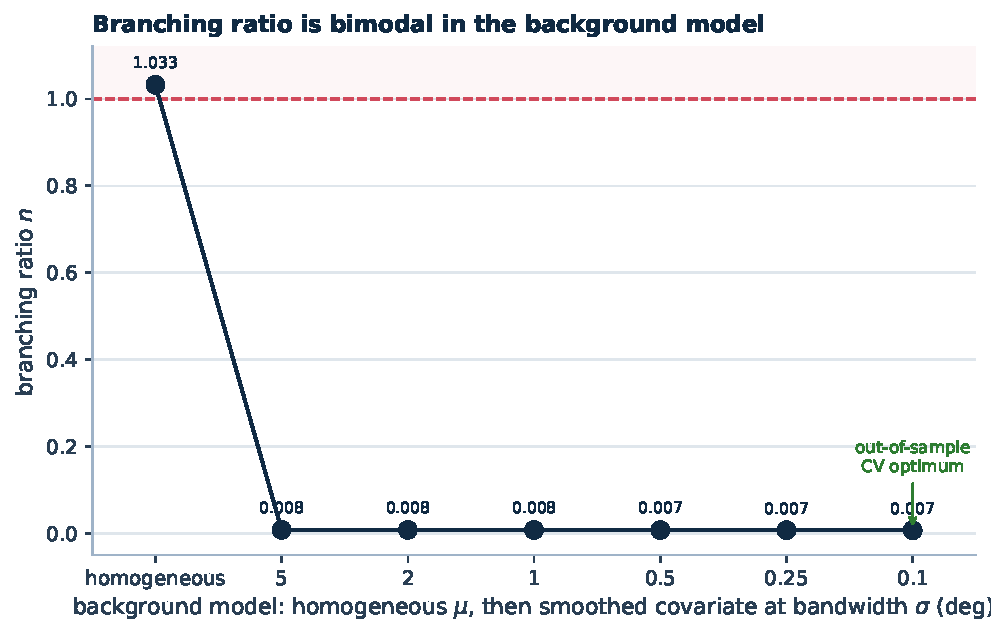
\includegraphics[width=0.85\textwidth]{figures/figure14_background_ladder.pdf}
\caption{H2, bimodal background dependence. Fitted branching ratio for the
homogeneous background and for smoothed-seismicity covariates of decreasing
bandwidth $\sigma$. Admitting any data-derived spatial background collapses $n$ from
$1.03$ to $\approx0$ ($\overline{P_{\mathrm{induced}}}\to0.99$); the held-out
cross-validation optimum is the most flexible (collapsed) background, not the
homogeneous one.}
\label{fig:ladder}
\end{figure}


\section*{Discussion}

\subsection*{Why the Shorter Window Performed Better}

The results support a descriptive conclusion: including earlier catalog decades
was associated with estimates on the other side of the stationarity boundary.
The 1960 fits used more than three times as many target events as the 2000 fit,
yet all were supercritical. Raising the threshold did not correct the problem,
and the tested perturbations to two starting values converged to the same local
solution. Catalog or seismicity nonstationarity is one hypothesis, not a result
established by this design.

Several mechanisms are plausible. Network coverage and magnitude practices have
changed since 1960. A fixed national $M_c$ cannot fully represent temporal and
spatial detection heterogeneity, and ETAS parameters are known to be sensitive
to truncation and missing events \citep{Seif2017,Mizrahi2021b}. A single
homogeneous background intensity must also explain a region spanning distinct
tectonic environments. The empirical background-location sampler captures
where inferred background events occurred, but it does not introduce
time-varying tectonic rates. Finally, a single stationary parameter vector must
represent decades containing major sequences and quieter intervals. The
shorter window may better match the post-2021 observation process and recent
rate regime, even though it has higher parameter uncertainty.

This interpretation does not imply that 2000 is an optimal start date. Among
the tested configurations at one origin, it produced the only point estimate
below unity and the smallest five-year count discrepancy after inspection of
the evaluation catalog. That post-selection comparison is exploratory. A
proper study should use many origins, hold auxiliary history fixed, cross
thresholds and starts factorially, and separate catalog-era effects from
individual sequences.

\subsection*{Consistency Is Not the Same as Skill}

The corrected N-test was consistent at three of five horizons, and the
resampled M-test at five of five. Aggregating these with conditional,
undersampled S- and PL-tests would be misleading. The horizons share most
observations, simulations were generated separately rather than as prefixes of
common five-year paths, and every model was inspected against the same
2021--2025 catalog. The reference comparison of
Figure~\ref{fig:reference} adds one comparative baseline and shows positive
spatial information gain for the admissible model, but a single reference at a
single origin is a weak skill statement.
Consistency asks whether an observation is plausible under a model; skill asks
whether one forecast predicts better than another. These are not equivalent
\citep{Zechar2010,Savran2022,Marzocchi2012}.

The first-year East Cape underforecast and subsequent overprediction illustrate
why horizon-resolved diagnostics matter. At one year the model missed a major
offshore sequence and underpredicted the national count by 145.5 events. By
three years, cumulative counts nearly matched. By five years, the model
overpredicted by 168.0 events. A single average count ratio or composite score
compresses this sign change and can obscure the process error.

\subsection*{Implications for Operational Forecasting}

Three safeguards follow directly from the run. First, the branching-ratio
point estimate and its uncertainty should be examined before simulation. The
override was useful diagnostically, but candidates whose uncertainty includes
or exceeds unity require an explicit constrained or finite-horizon
formulation. Second, maximum
magnitude must be specified or inferred from a defensible tapered distribution.
An $M11.2$ realization is not a useful expression of epistemic uncertainty for
this domain. Third, spatial background structure should be tested against an
independent long-term model rather than inferred only from the same catalog used
to fit triggering.

Parameter uncertainty is now quantified for the branching ratio
(Fig.~\ref{fig:uncertainty}) but is not yet propagated into the forecast
ensembles, which still condition on one fitted parameter vector. The asymptotic
M-step interval is conditional on the converged background probabilities; a
parametric bootstrap, full profile likelihood, or Bayesian posterior would be a
stronger basis, and the forecast distribution should ultimately integrate over
the parameter uncertainty. That refinement matters here because the 2000-window
interval reaches the stationarity boundary and the 1980-window interval crosses
it, so the admissibility of the borderline configurations is not resolved by a
single fit.

\subsection*{Limitations}

This analysis has eight principal limitations. (1) The forecast evaluation uses
one retrospective origin and cannot establish prospective performance; the
branching-ratio behavior was checked at five origins
(Fig.~\ref{fig:origins}), but the calibration, spatial, and magnitude diagnostics
were not. (2) Horizons are nested, so cross-horizon pass counts and calibration
statistics are dependent. (3) The sweep explored only seven nonfactorial
configurations. (4) Fixed completeness thresholds were assumed, and reported
magnitudes were not homogenized: the catalog mixes at least seven magnitude
types (predominantly $M_L$, with $M_w$, $m_B$, $M_{Lv}$, and unspecified
entries), whose systematic differences are not corrected here and would shift
both $M_c$ and $\beta$. (5) The forecast simulations include no maximum
magnitude, fault geometry, or depth dependence, and although branching-ratio
uncertainty is now estimated (Fig.~\ref{fig:uncertainty}) it is not propagated
into the ensembles. (6) Training and auxiliary-history starts changed together.
(7) The source domain is truncated at $180^\circ$ E, immediately west of the
East Cape sequence; the GeoNet catalog contains about 2{,}730 $M\geq4$ events in
$180^\circ$--$184^\circ$ E within the latitude band (1{,}156 of them in the
2000--2021 window at $M\geq4.1$, a 20\% addition to that training set).
Refitting the 2000-window model on a buffered, dateline-aware domain
($165^\circ$--$184^\circ$ E, longitudes unwrapped so the great-circle distances
remain valid) raises its branching ratio from 0.969 to 1.000 (95\% interval
$[0.971,1.029]$), erasing the only subcritical classification in the sweep. The
admissibility of the 2000-window fit is therefore partly an artifact of the
truncated domain, and a dateline-aware re-run of the full spatial and calibration
analysis is required. (8) Random
seeds were not fixed, although 2,000 archived realizations limit Monte Carlo
error for common probabilities.

There is also a reproducibility distinction between data and experiment state.
The GeoNet catalog is continually revised, and a fresh query may not reproduce
the exact input file. The archived \texttt{nzcat.csv}, parameter files,
simulation catalogs, and software revision are therefore part of the
computational record. Future experiments should version the catalog query,
record event-product revisions, and use deterministic seed sequences.

\section*{Conclusions}

A New Zealand-wide ETAS calibration sweep found a strong association between
tested catalog windows and fitted branching ratios. The five 1960-start
configurations were significantly supercritical (95\% intervals wholly above
unity); the 2000-window fit was significantly but marginally subcritical
(profile-likelihood interval $[0.944,0.995]$); and the intermediate 1980-window
fit sat essentially exactly on the stationarity boundary, its asymptotic interval
including unity and its profile interval marginally excluding it. Refitting at four
additional origins confirmed that the long windows are supercritical at every
origin while the 2000 window is subcritical at four of five, crossing the
boundary at the Kaikoura-dominated 2017 origin. The 2000-window ensemble
strongly underpredicted first-year counts, shifted to longer-term
overprediction, placed its largest residual on the truncated East Cape boundary,
and generated implausible upper-magnitude realizations under its unbounded
Gutenberg--Richter law---though it carried positive spatial information beyond a
smoothed-seismicity reference.

The appropriate conclusion is not that the 2000-window model is validated for
operations. Rather, the experiment demonstrates a reproducible screening
workflow: estimate the branching ratio with its uncertainty and reject or
constrain inversions whose interval reaches unity, inspect calibration as a
function of horizon and location, impose a defensible magnitude tail, score
against a reference, and repeat at independent forecast origins. Those steps are
necessary before the apparent consistency of a catalog ensemble can be
interpreted as forecast skill.

The six mechanism tests sharpen this further. They show that a fitted branching
ratio above unity, for a national catalog assembled this way, is not by itself
evidence that the seismicity is supercritical: the same number can be produced by
the observation process acting on a subcritical truth, by withholding spatial
background structure the data prefer out-of-sample, by pooling tectonically
distinct depth regimes, or by an accident of where the domain boundary falls
relative to one sequence. We therefore recommend that the branching ratio be
reported not as a scalar but as a robustness profile across these choices, and
that the horizon-slope diagnostic accompany the standard consistency tests as an
early screen for criticality miscalibration.

\section*{Data and Resources}

The earthquake catalog was obtained from the GeoNet FDSN event service at
\url{https://service.geonet.org.nz/fdsnws/event/1/query} (last accessed June
2026). The analysis and experiment code are in the project repository at
\url{https://github.com/KennyGraham1/lmizrahiEtas}: the primary sweep analysis is
\nolinkurl{examples/bssa_nz_wide_calibration/analyze_sweep.py}, and the follow-up
analyses (branching-ratio asymptotic and profile-likelihood intervals, the
multiple-origin and dateline-aware refits, the homogenized refit, the
bounded-magnitude comparison, and the smoothed-seismicity reference) are in
\nolinkurl{examples/bssa_nz_wide_calibration/experiments/}, with figures and
tables produced by \nolinkurl{analyze_experiments.py}. The six mechanism tests
(figures~9--14) are produced by, respectively,
\nolinkurl{synthetic_injection.py} (H1, with the matched and uniform
configurations), \nolinkurl{background_ladder.py} (H2),
\nolinkurl{sequence_dominance.py} and \nolinkurl{sequence_dominance_drivers.py}
(H3), \nolinkurl{depth_stratified.py} (H4), \nolinkurl{boundary_flux.py} (H5),
and \nolinkurl{calibration_slope.py} (H6), with their figures assembled by
\nolinkurl{figures_hypotheses.py}. \textbf{[Before
submission, the authors will tag a release whose commit contains all of the
above code and cite that tag/commit here; the current draft hash predates the
follow-up analyses.]} The exact input catalog (\nolinkurl{nzcat.csv} and the
buffered, homogenized variant), inversion outputs, evaluation metrics, and the
approximately 4.2~GB simulation archive will be deposited in a permanent
repository with checksums, environment metadata (Python and package versions),
and a DOI before submission; random-seed sequences will be fixed in that
deposited version so the simulations are bitwise reproducible. pyCSEP version
0.8.0 was used for catalog evaluations.

In accordance with SSA policy, we disclose that generative artificial
intelligence tools assisted in preparing this article. Specifically, a large
language model assisted with drafting and editing the manuscript text and with
implementing the analysis, the follow-up experiments (branching-ratio
uncertainty, multiple-origin refits, the bounded-magnitude and reference-forecast
comparisons, the dateline-aware refit, and the six mechanism tests of
Figures~\ref{fig:synthetic}--\ref{fig:ladder}), and the figure-generation code in
the cited repository, and with cross-checking bibliographic records. All reported
numerical results were produced by executing this documented code rather than by
the model directly. The authors reviewed and verified all code, analyses,
figures, citations, and conclusions and take full responsibility for the content.
\textbf{[Authors: before submission, replace this bracketed note with the exact
tool name(s), version and extension numbers, and manufacturer(s) used---for
example the specific assistant product and release---as SSA requires naming the
tool and its manufacturer.]}

\section*{Declaration of Competing Interests}

The authors declare no competing interests.

\section*{Acknowledgments}

The authors thank GeoNet and GNS Science for maintaining the New Zealand
earthquake catalog. Funding sources and contributor acknowledgments must be
added by the authors before submission.

\bibliographystyle{apalike}
\bibliography{references}

\end{document}
